\subsection{Analyses and Discussions}
\hanna{In this section you might want to discuss some qualitative results and error analyses; For example, Rationales requiring background knowledge can be part of error analyses. Do not frame this as a future direction because it sells the work as it is in progress. }
Our exploration into scientific claim verification has revealed a number of promising future research directions to improve data collection, modeling, and integration with complementary tools for scientific literature.

%%%%%%%%%%%%%%%%%%%%

\paragraph{Partial evidence}

In Figure \ref{fig:partial}, the abstract contains evidence relevant to the given claim, but the context is different (mouse vs. human). In pilot experiments, we instructed annotators to label cases of context mismatch as \spart / \rpart, and to \emph{edit} the given claim such that the evidence matched context of edited claim (see \citet{Min2020AmbigQAAA} for a related approach applied to information-seeking questions). Unfortunately, inter-annotator label agreement was only \labelkappafine Cohen's $\kappa$ due to disagreement over the \ppartial label. We hope to refine the annotation task and improve annotator agreement in the future.

\begin{figure}[t]
  \centering
  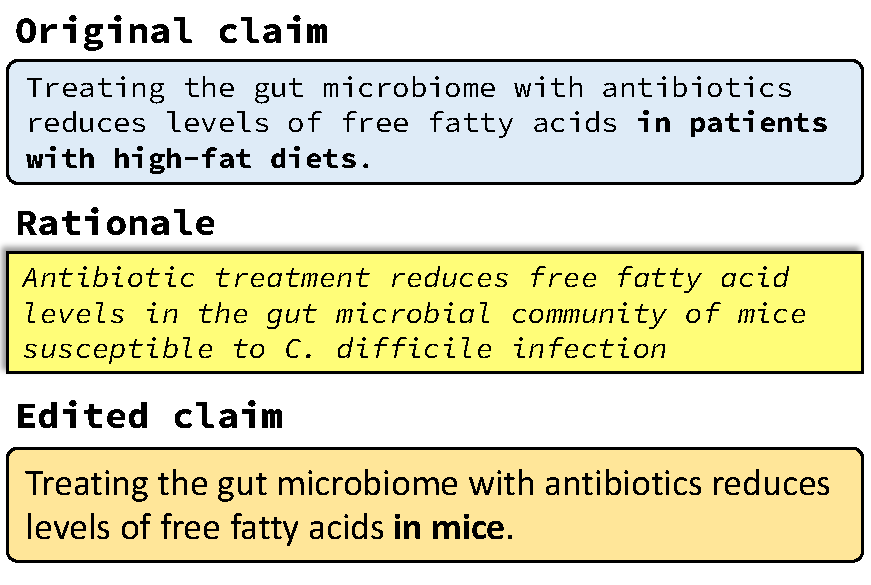
\includegraphics[width=\columnwidth]{figures/partial-fig.pdf}

  \caption{An abstract that partially supports a claim. The edited claim is fully supported.}
  \label{fig:partial}
\end{figure}

%%%%%%%%%%%%%%%%%%%%

\paragraph{Rationales requiring background knowledge}

In principle, a rationale should provide standalone justification for a model's prediction. But what if the rationale relies on the context established by the rest of the document, or never stated explicitly at all? For instance, the rationale excerpted in Figure \ref{fig:teaser} never mentions that Citalopram is an antidepressant, but this fact is required to justify the model's decision. Future work could explore integrating external knowledge sources like  \emph{abstractive rationales} which summarize the context or background knowledge necessary for a claim to follow from a given \emph{extractive} rationale.

%%%%%%%%%%%%%%%%%%%%

\paragraph{Evidence credibility and synthesis}

The system developed in this work identifies linguistic relationships between claim and evidence, but does not attempt to assess the credibility of the evidence itself.



Our system could be fruitfully combined with tools like the recently-created Scite.AI platform\footnote{https://www.scite.ai}, which assesses the strength of the results reported in a scientific article by examining the \emph{intent} of citations citing this article. In addition, claim verification systems could serve as a component in automated evidence synthesis frameworks (\S\ref{sec:related_work}), which could weight individual \supports\ / \refutes labels by the strength of their evidence documents to arrive at a corpus-level verdict.

%%%%%%%%%%%%%%%%%%%%
